\section{Modele dyskretne}
\subsection{Równania stanu}
Na podstawie modelu ciągłego opracowano następujący model dyskretny:
\begin{align*}
 x_1(k)= &\left[ u_1(k-1) + u_2(k-1-\frac{\tau_c}{T_p}) + v_1(k-1) - \alpha \left( \frac{x_1(k-1)}{C} \right)^{0.25} \right]T_p +x_1(k-1)\\
\begin{split} x_2(k) =& 
 \bigg[ T_H \cdot u_1(k-1) + T_C \cdot u_2(k-1-\frac{\tau_c}{T_p}) + T_D \cdot v_1(k-1) +\\ & -\left( u_1(k-1) + u_2(k-1-\frac{\tau_c}{T_p}) + v_1(k-1) \right)\cdot x_2(k-1) \bigg]T_p \cdot x_1^{-1} (k-1)  +x_2(k-1)\end{split} \\\\
 y_1(k) = &\sqrt{\frac{x_1}{C}} \\\\
 y_2(k) =  &x_2(k-\tau)
\end{align*}




Dokonano linearyzacji w punkcie pracy $p = (\overline{u_1}, \overline{u_2}, \overline{v_1}, \overline{x_1}, \overline{x_2} )$:

\begin{align*}
\begin{split}
x_1(k) = &\left[ \overline{u_1} + \overline{u_2} + \overline{v_1} - \alpha \left( \frac{\overline{x_1}}{C} \right)^{0.25} \right]T_p + \overline{x_1} + T_p \left( u_1(k-1) - \overline{u_1} \right) +T_p\left( u_2(k-1 - \frac{\tau_c}{T_p}) - \overline{u_2} \right)+ \\ &+ \left( - \alpha Tp \frac{\overline{x_1}^{0.25}}{4 C^{0.25} x_1 } +1 \right)(x_1(k-1) -\overline{x_1})
\end{split}\\
\begin{split}
x_2(k) = &\bigg( T_H \overline{u_1} + T_C \overline{u_2} + T_D \overline{v_1} - (\overline{u_1}+\overline{u_2}+\overline{v_1})\overline{x_2} \bigg)\overline{x_1}^{-1}T_p + \overline{x_2} + \frac{T_p(T_H-\overline{x_2})}{\overline{x_1}}(u_1(k-1)-\overline{u_1})  + \\ &+ \frac{T_p(T_C-\overline{x_2})}{\overline{x_1}}\left(u_2(k-1-\frac{\tau_c}{T_p})-\overline{u_2}\right)+
\frac{T_p(T_D-\overline{v_1})}{\overline{v_1}}(v_1(k-1)-\overline{v_1}) + \\ &-\frac{T_p}{\overline{x_1}^2}\left( T_H \overline{u_1} + T_C \overline{u_2} + T_D \overline{v_1} - (\overline{u_1}+\overline{u_2}+\overline{v_1})\overline{x_2} \right)(x_1(k-1)-\overline{x_1}) +\\ &+
\left(\frac{-T_p}{\overline{x_1}}(\overline{u_1}+\overline{u_2}+\overline{v_1}) +1\right)(x_2(k-1)-\overline{x_2}) 
\end{split}\\
y_1(k) = &\sqrt{\frac{\overline{x_1}}{C}}+\frac{1}{2\sqrt{\overline{x_1}C}}(x_1(k)-\overline{x_1})\\
y_2(k) = &  x_2(k-\tau)
\end{align*}

\newpage

\subsection{Transmitancje}
 Przyjęto czas próbkowania $T_p = 0.1s$, korzystając z uprzednio wyliczonego w Matlabie modelu ciągłego a także polecenia \emph{c2d()} wyliczono następujące transmitancje:
 
 \begin{align*}
\frac{U_1}{Y_1} &= \frac{0.003995}{z - 0.9976} \\
\frac{U_1}{Y_2} &= z^{-400} \cdot \frac{0.004516 z - 0.004506}{z^2 - 1.997 z + 0.9966} \\
\frac{U_2}{Y_1} &= z^{-1000}\frac{0.003995}{z - 0.9976} \\
\frac{U_2}{Y_2} &= z^{-1400} \cdot \frac{-0.002587 z + 0.002581}{z^2 - 1.997 z + 0.9966} \\
\frac{V_1}{Y_1} &= \frac{0.003995}{z - 0.9976} \\
\frac{V_1}{Y_2} &= z^{-400} \cdot \frac{-0.001009 z + 0.001006}{z^2 - 1.997 z + 0.9966} \\
 \end{align*}
 
\subsection{Porównanie modelu ciągłego z dyskretnym}

Zarejestrowano odpowiedzi skokowe modelu ciągłego i modeli dyskretnych o różnym czasie próbkowania. Wyniki tych doświadczeń przedstawiono na poniższych wykresach. 

\begin{figure}[H]
    \centering
    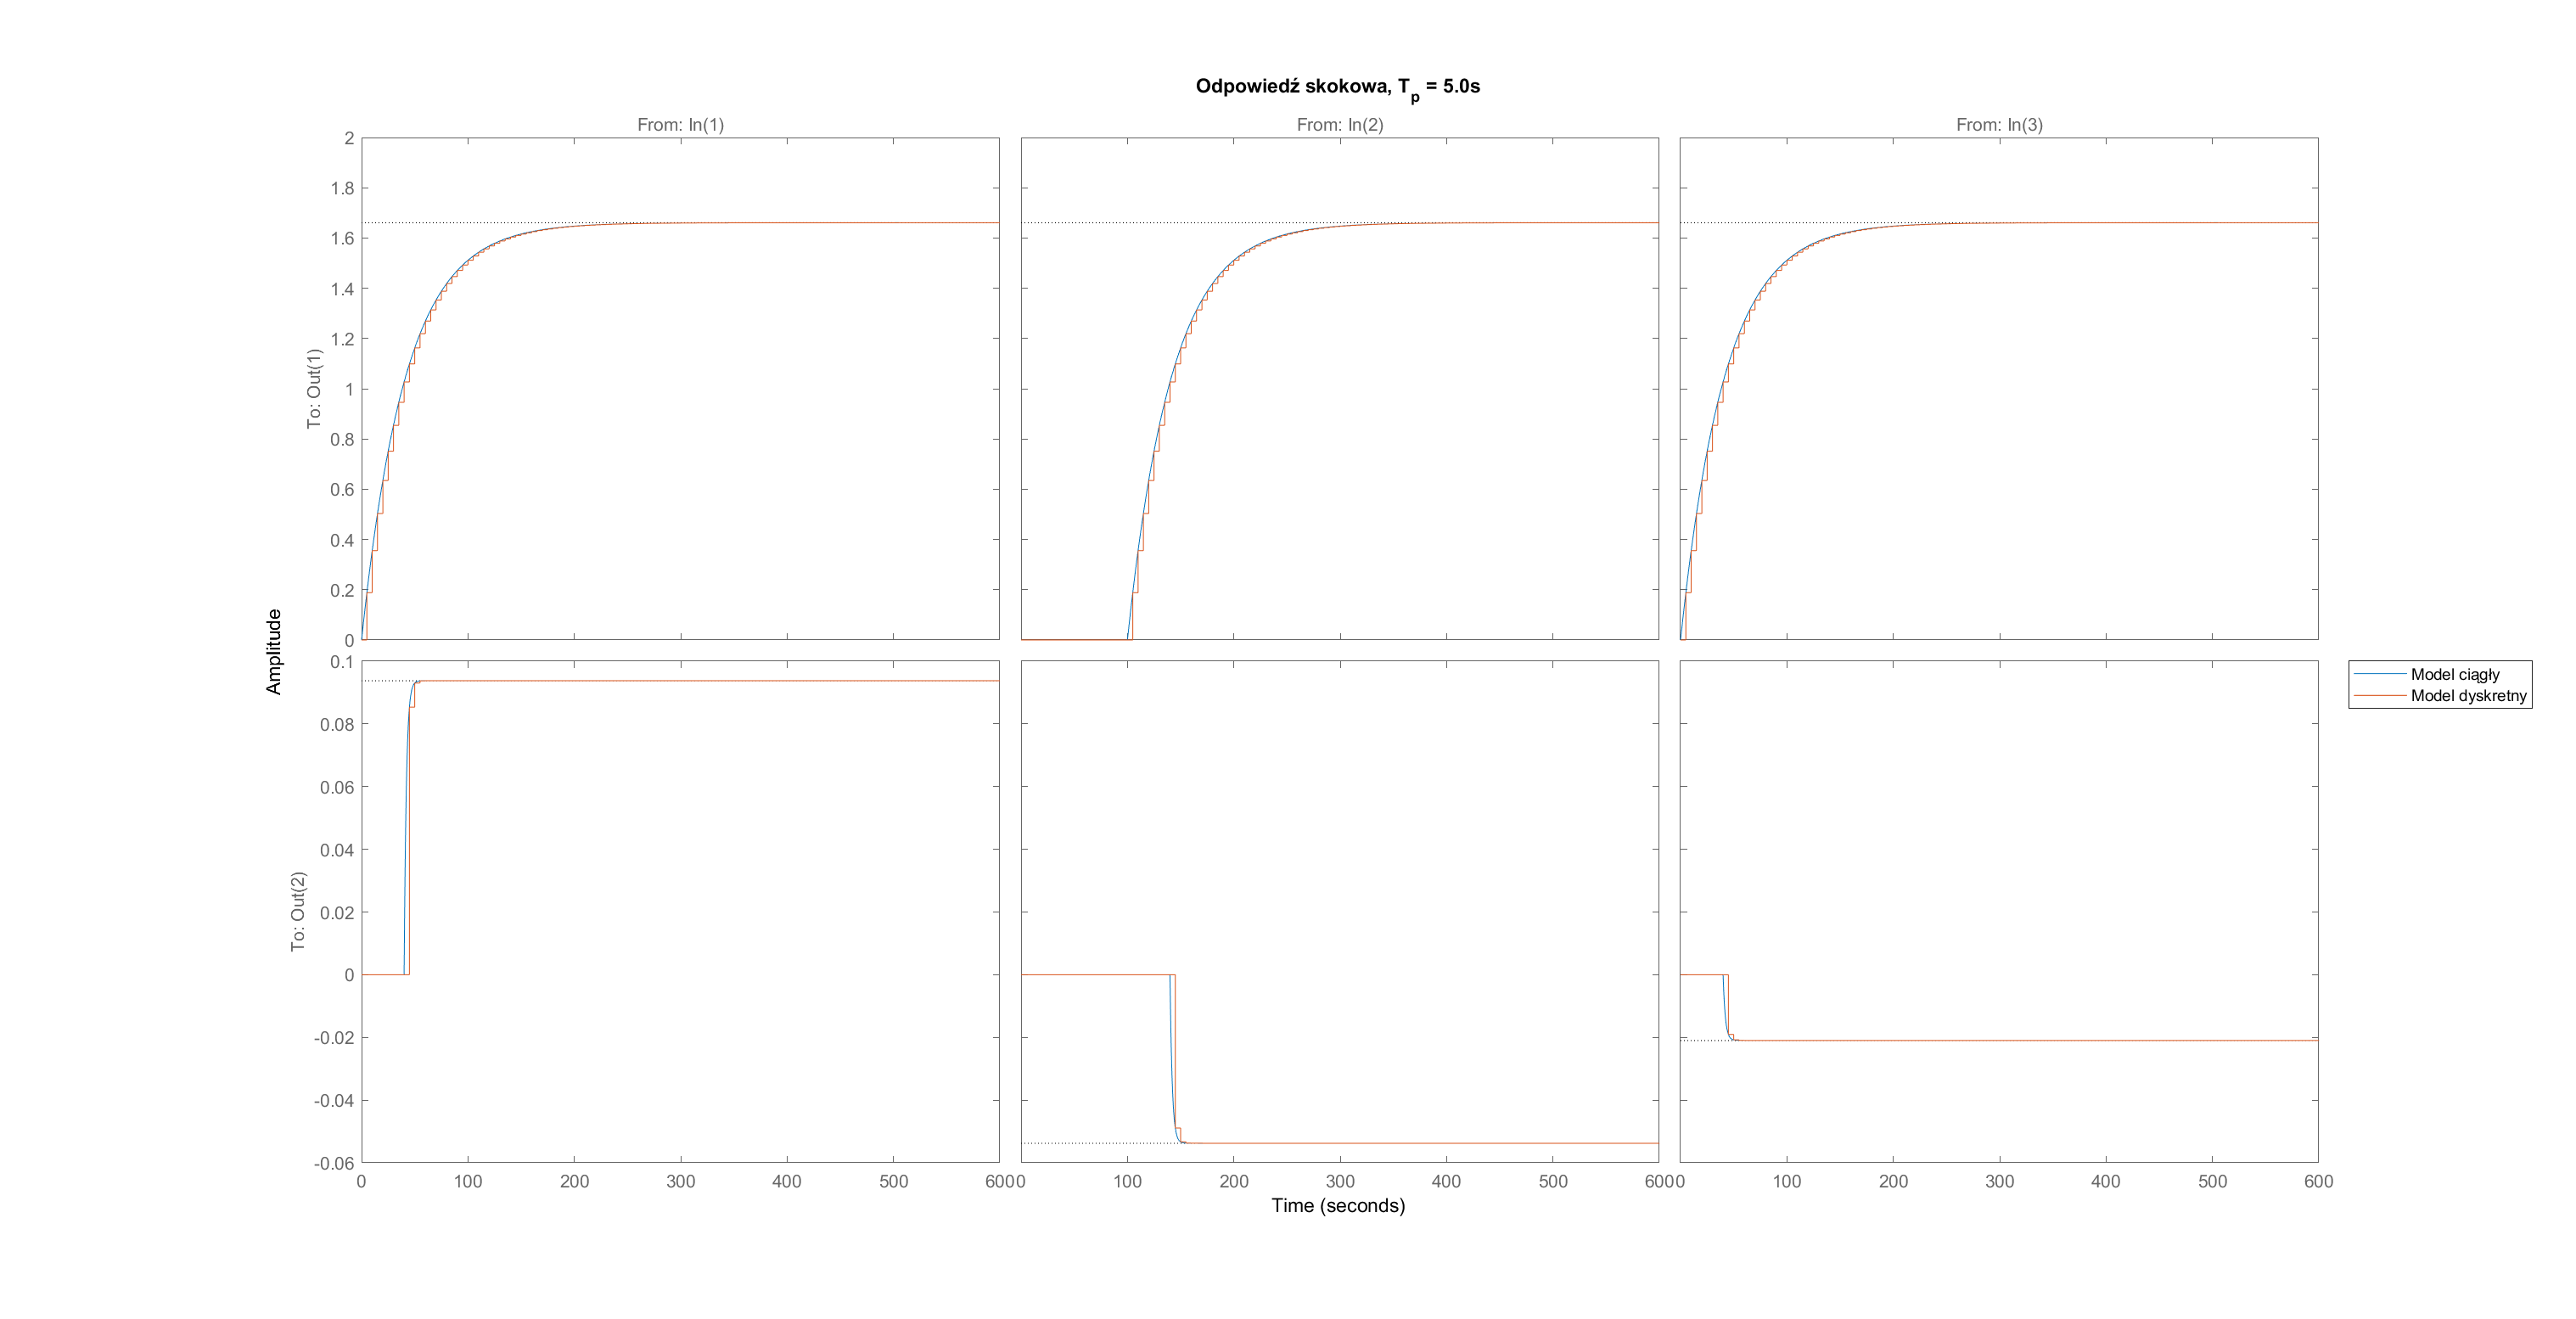
\includegraphics[scale=0.35]{images/stepdt5_00.eps}
    \caption{Odpowiedzi skokowe modeli}
\end{figure}

\begin{figure}[H]
    \centering
    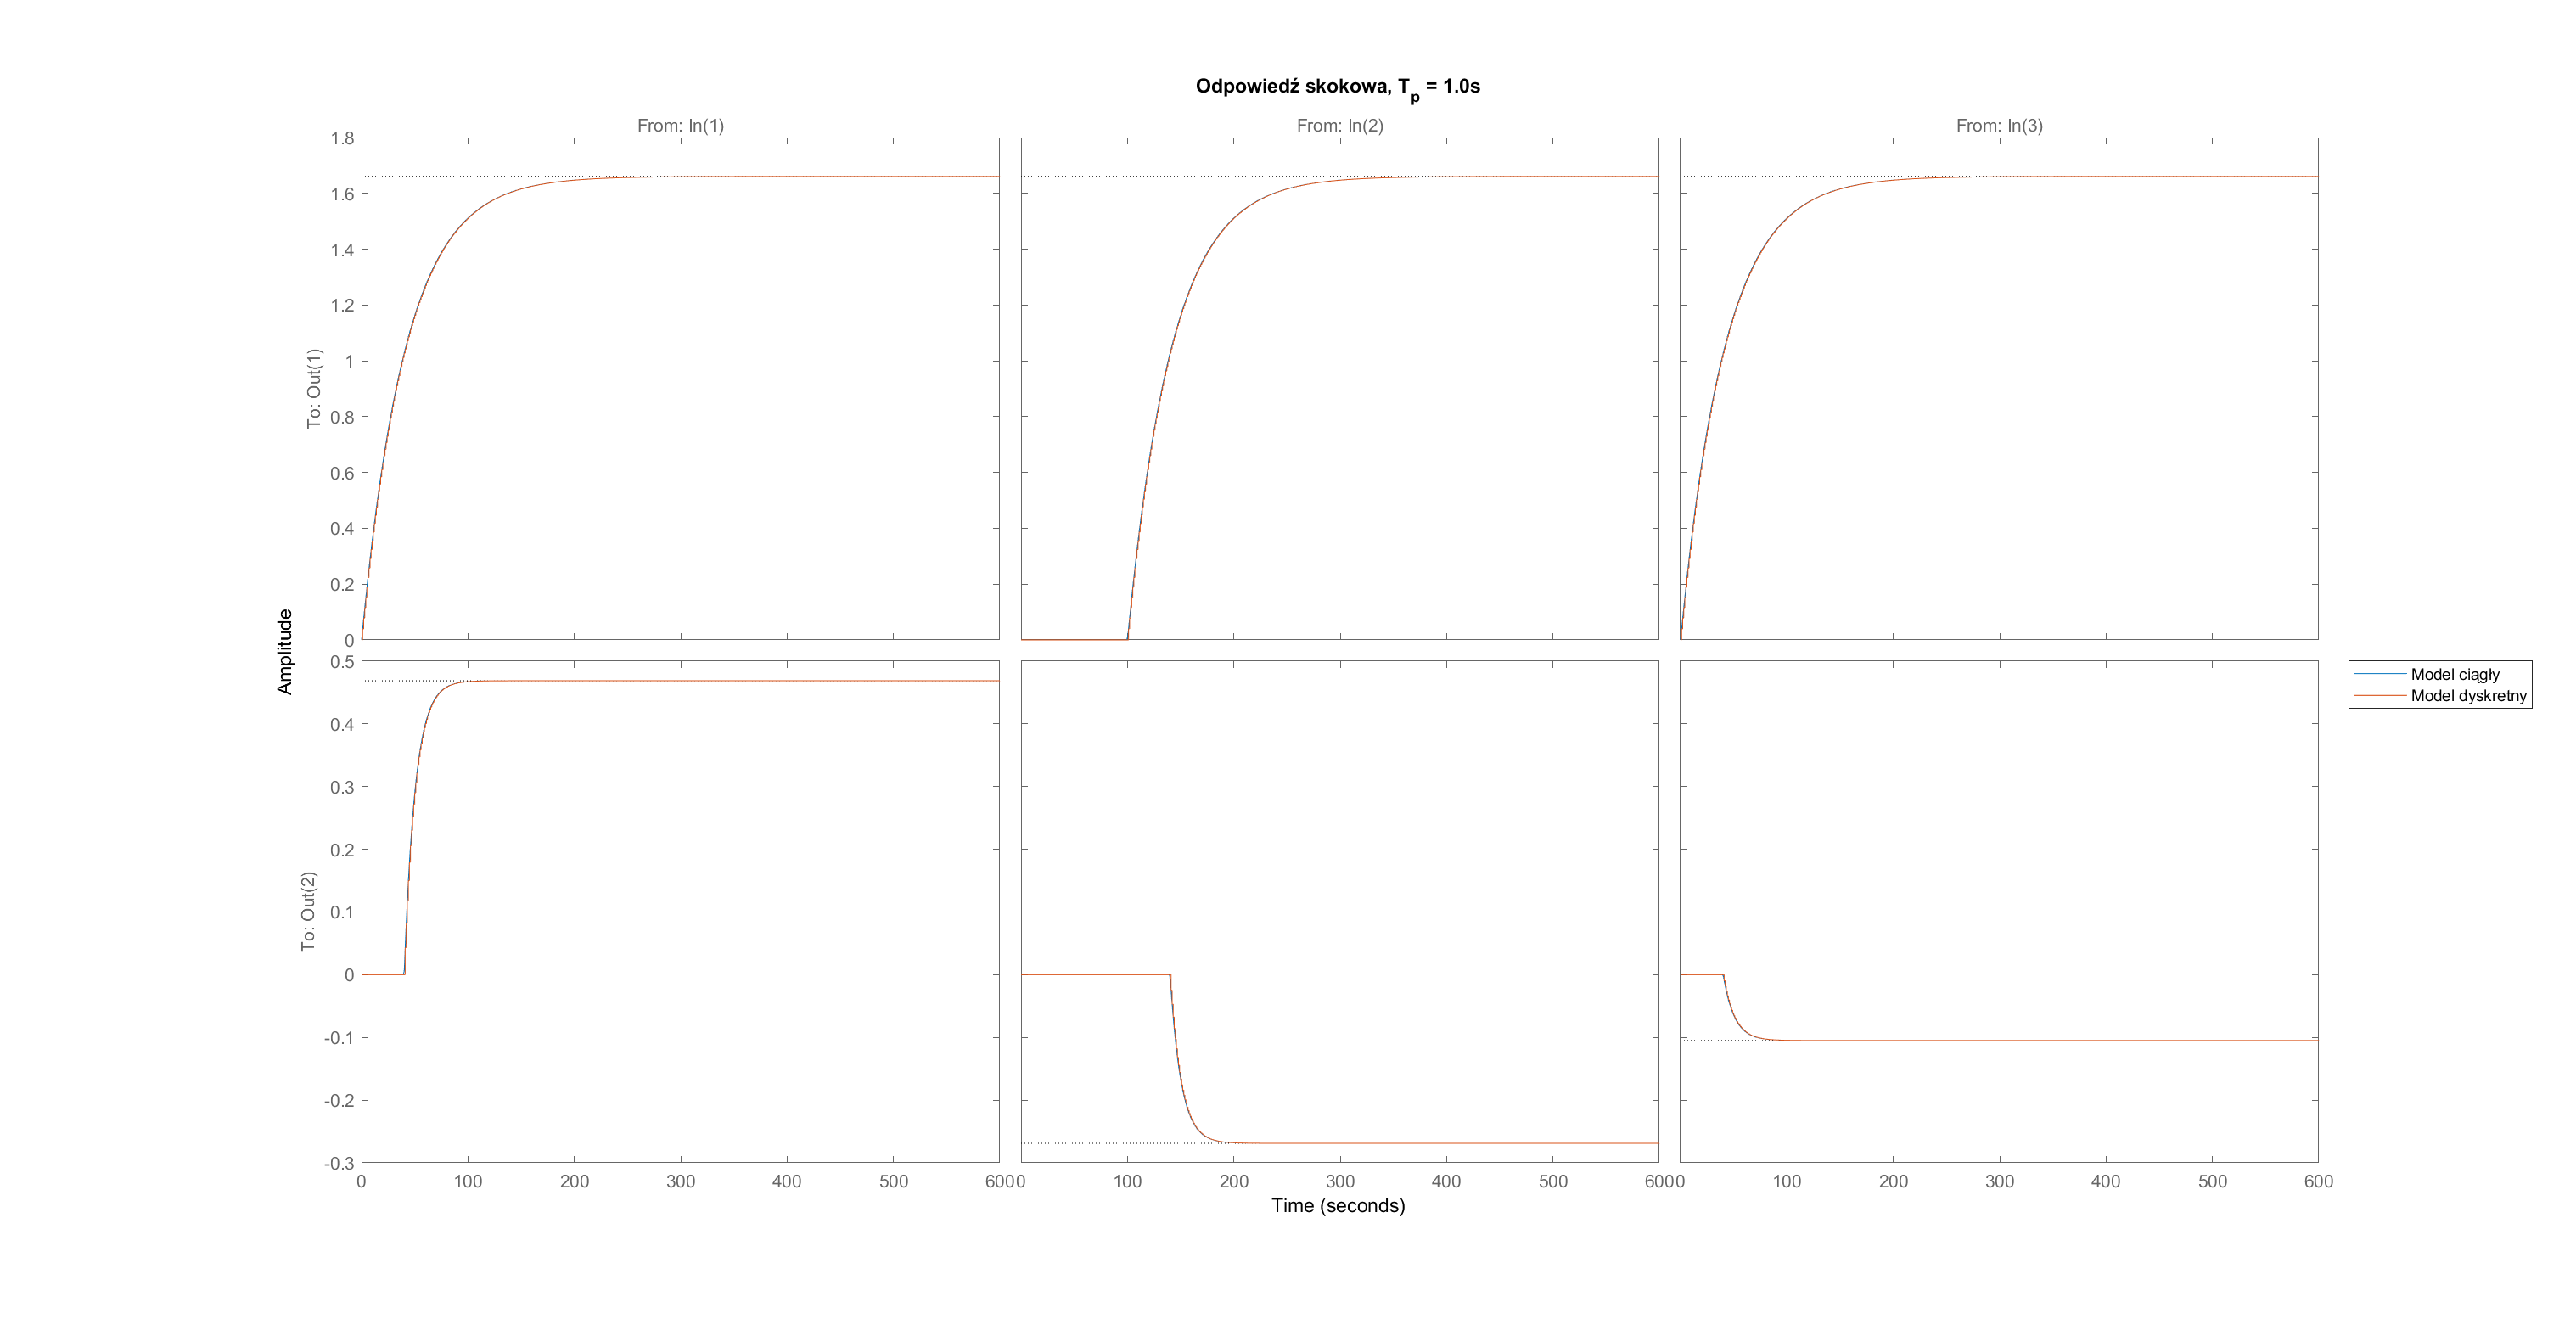
\includegraphics[scale=0.35]{images/stepdt1_00.eps}
    \caption{Odpowiedzi skokowe modeli}
\end{figure}

\begin{figure}[H]
    \centering
    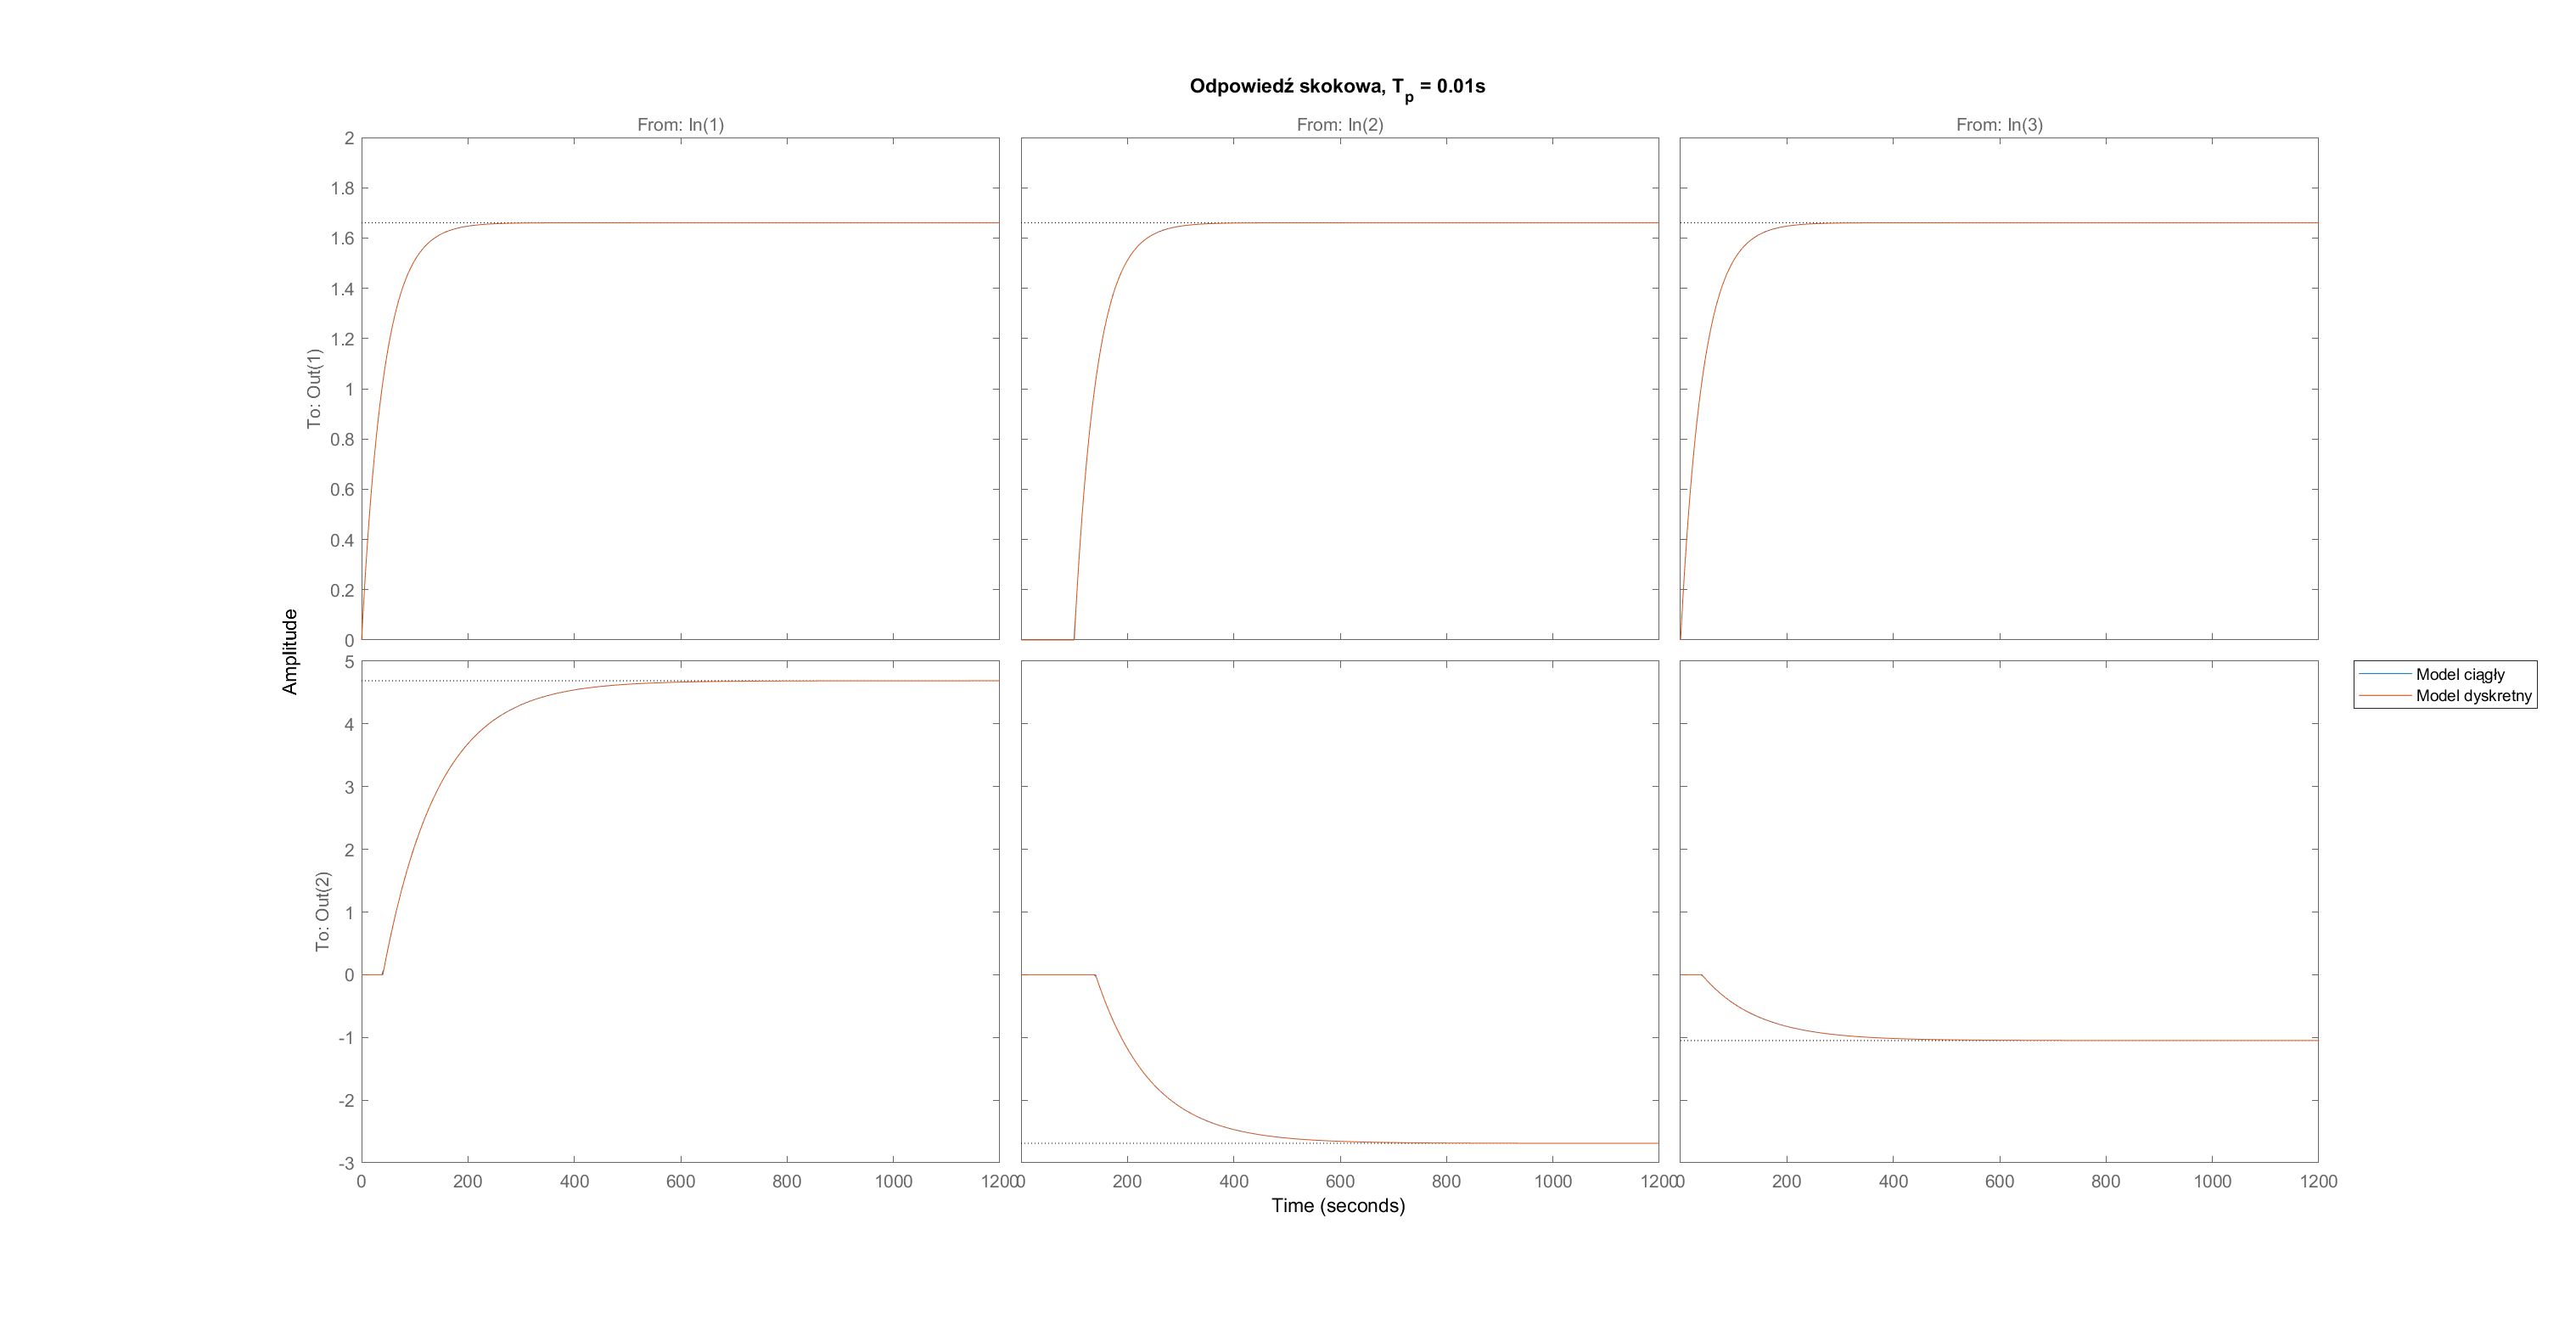
\includegraphics[scale=0.35]{images/stepdt0_01.eps}
    \caption{Odpowiedzi skokowe modeli}
\end{figure}

Z wykresów wyraźnie wynika, że jest konieczny odpowiedni mały krok dyskretyzacji ze względu na szybkie tempo zmian w procesie, stąd też zdecydowano się na krok dyskretyzacji $T_p = 0.1s$.